% ------------------------------------------------------------------------
% ------------------------------------------------------------------------
% ------------------------------------------------------------------------
%\chapter{MCQMC 2012}



\chapter{Practical Information}



\section{Conference Venue}
MCM 2025 is hosted by Illinois Institute of Technology (Illinois Tech).  All talks will take place on the Mies Campus in the following three buildings
\begin{itemize}
	\item Hermann Hall (HH),
	\item Perlstein Hall (PH), and
	\item Wishnick Hall(WH)
\end{itemize}
See the campus map on the next page or at \href{https://www.iit.edu/sites/default/files/2022-08/mies-campus-accessibility-map-2022.pdf}{this link}.  

The registration desk, the coffee breaks, and the Monday night welcome reception will all be  in the Hermann Hall Lobby.

\clearpage

\begin{center}
	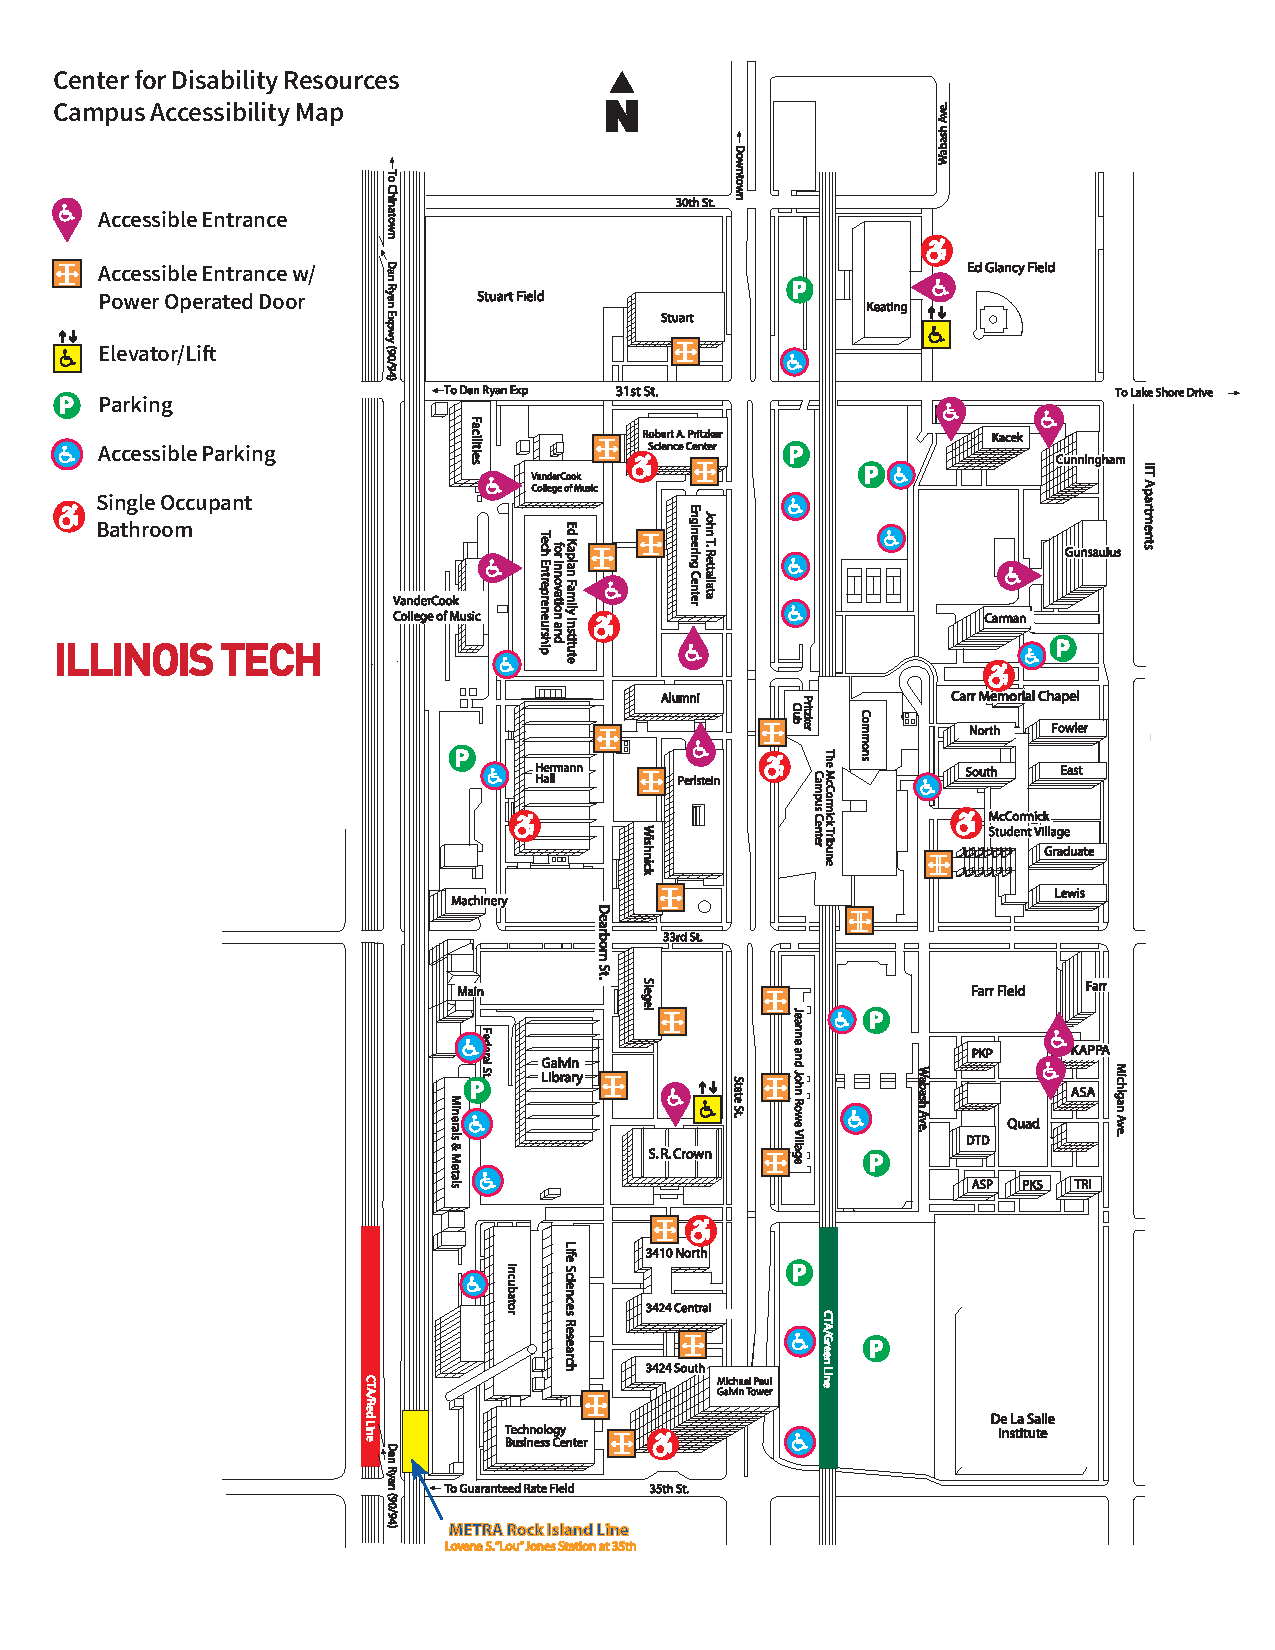
\includegraphics[width = \textwidth] {Photos/mies-campus-accessibility-map-2022.pdf}
\end{center}



\begin{center}
	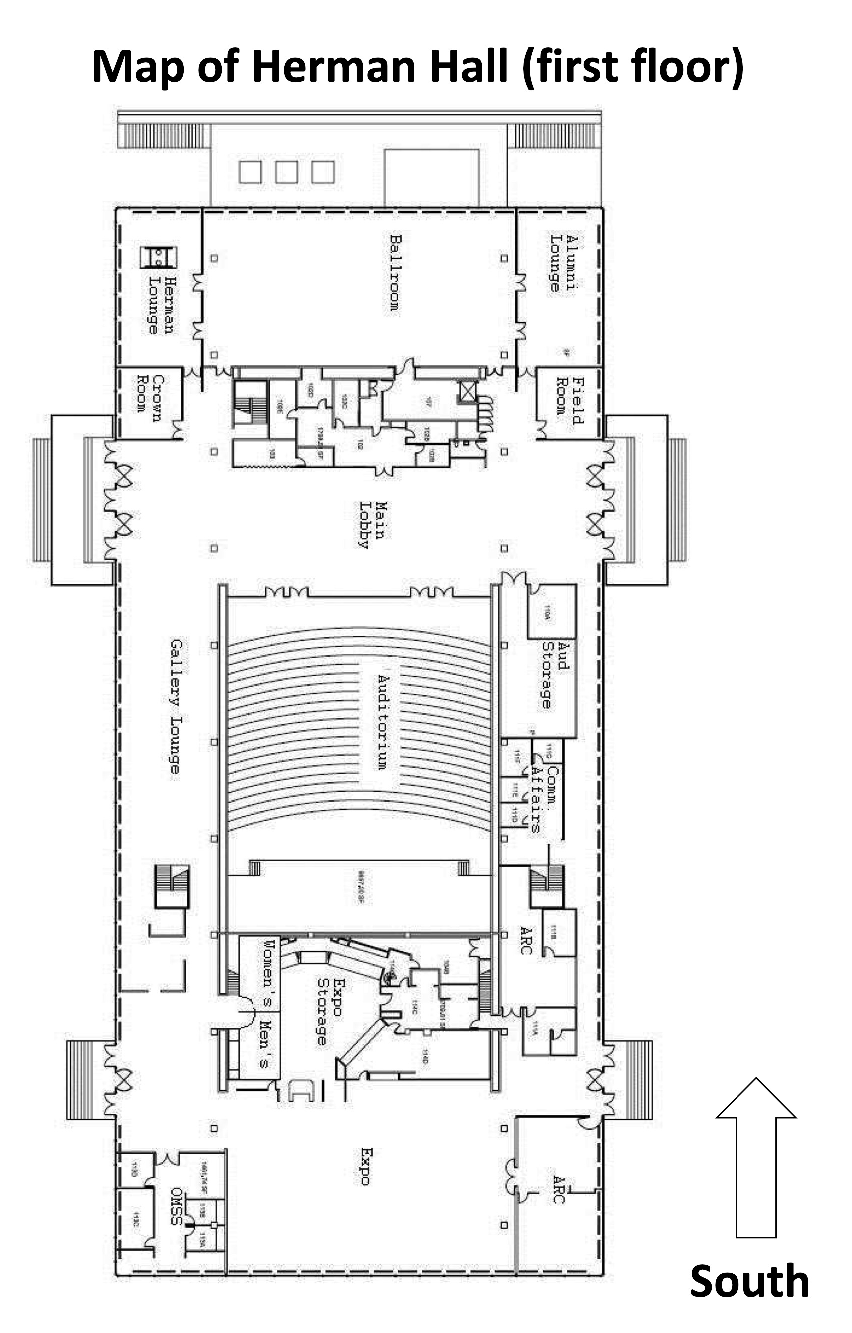
\includegraphics[width =0.95 \textwidth] {Photos/MapHermannHallFirstFloor_cropped.eps}
\end{center}
\clearpage

\section{Getting to Illinois Tech}

\subsection{Local Transportation}
Illinois Tech is located several miles south of downtown.  You  can reach Illinois Tech via 
\begin{itemize}
	\item the Chicago Transit Authority (\href{https://www.transitchicago.com/schedules/}{CTA}) `L' Green or Red Lines, which stop at 35th Street, 
	\item the href{https://www.transitchicago.com/schedules/}{CTA} Route 29 bus, which stops at the corner of State and 32nd Streets, or
	\item taxi, Uber, or Lyft.
	 \item If you are driving to Illinois Tech, there is paid visitor parking in the lot on the east side of State Street between 31st and 32nd Streets (enter via State Street).
\end{itemize}

\subsection{Getting to Chicago}

\begin{itemize}
  \item Two major airports, \href{https://www.flychicago.com/ohare/home/Pages/default.aspx}{O'Hare} and \href{https://www.flychicago.com/midway/pages/default.aspx}{Midway} serve Chicago, and are not far from Illinois Tech.  
  \item Our main domestic passenger rail line is \href{Amtrak}{https://www.amtrak.com/home.html}.
\end{itemize}




\section{Food}

Meals will \emph{not} be provided, except for the Wednesday night conference banquet. There are several places on campus or nearby where you can purchase meals.  They are show in \href{https://www.google.com/maps/d/u/1/edit?mid=1QH5guZDg-m8_f1oO9HgZ5sIL76q1gdk&usp=sharing}{this map}


\arrayrulecolor{black}

\begin{center}
 \begin{longtable}{|| l || l | l | l l||} 
 \hline
 \hline  
  \textbf{JKU Mensa}  & \url{www.mensen.at}  & Mon--Fri & 11:00--13:30  \\ \hline
  1B & \textbf{Cafe Ch@t} & Keplergeb\"{a}ude &  Mon--Thu & 08:00--19:00 \\
     &                    &                         &  Fri & 08:00--14:00 \\ \hline
  1C & \textbf{Science Cafe} & Science Park 3 &  Mon--Thu & 08:00--16:00 \\ 
     &                    &                         &  Fri & 08:00--14:00 \\ \hline
  1D & \textbf{Cafe Sassi} & Bankengeb\"{a}ude &  Mon--Thu & 08:00--16:00 \\
     &                    &  \url{www.sassi.at}  &  Fri & 08:00--14:00 \\ \hline
  1E & \textbf{Teichwerk} & University pond &  Mon--Thu & 08:00--16:00 \\
     &                    & \url{www.dasteichwerk.at}  &  Fri & 08:00--14:00 \\ \hline
  2  & \textbf{KHG Mensa} & Mengerstr. 23 & Mon--Fri & 11:00--13:00  \\ 
  
     &                    & \texttt{https://www.dioezese-linz.at/} & & \\
     &                    &  \texttt{khg/mensa/menueplan}  & & \\ \hline
  3  & \textbf{Winklermarkt} &  Altenbergerstr. 40 & Mon--Thu & 07:30--18:30 \\
     & (Supermarket \& &  \texttt{https://winklermarkt.at/}  & Fri & 07:30--19:00 \\
     & Restaurant) &  \texttt{menuplan/}  & Sat & 07:30--17:00 \\ \hline
  4a  & \textbf{Pizzeria} & Aubrunnerweg 1a & Mon--Sun & 11:00--15:00 \\
     & \textbf{Bella Casa} & Phone: +43-732-245646 &          & 17:00--24:00 \\ \hline
  4b  & \textbf{Chinese Restaurant} & Aubrunnerweg 11 & Mon--Sun & 11:00--14:30 \\
     & \textbf{Jadegarten} & Phone: +43-732-750160 &          & 17:00--23:00 \\ \hline
  5  & \textbf{Restaurant} & Altenbergerstr. 6--8 & Mon--Thu & 10:30--22:00 \\
     & \textbf{Burgerista} &  Phone: +43-50-666666 &  Fri--Sat & 10:30--23:00 \\ 
     &  &                     &  Sun & 10:30--23:00 \\ \hline
  6  & \textbf{Restaurant} & Freist\"{a}dter Str. 297 & Mon--Sat & 11:00--23:00 \\
     & \textbf{Peter's Platz} &  Phone: +43-732-251112                   &  Sun & 11:00--17:00 \\ \hline
  7 & \textbf{Subway} & Freist\"{a}dter Str. 313 & Mon--Sun & 11:00--22:00 \\ \hline
  8  & \textbf{Asian Restaurant} & Freist\"{a}dter Str. 315 & Tue & 11:30--14:30 \\
     & \textbf{Ost18} &  Phone: +43-732-244042              &  Wed--Mon & 11:30--14:30 \\ 
     &  &   &   & 17:30--23:00 \\ \hline
  9  & \textbf{Raab Mensa} & Julius-Raab-Str. 10 & Bar: & \\
     & (Restaurant \& Bar)   & Phone: +43-732-24570 & Mon--Thu & 06:30--23:30\\
     &             & \texttt{www.sommerhaus-hotel.at/} & Sat--Sun & 06:30--11:00 \\
     &                            & \texttt{de/linz\#{}speiseplan} & Restaurant:& \\
     &                            &  & Mon--Sun & 11:30--14:30\\
     &                            &  &  & 17:00--21:00\\ \hline
 10  & \textbf{McDonald's \&} & Freist\"{a}dter Str. 298 & Sun--Thu & 07:00--00:00 \\
     & \textbf{McCafe} &               &  Fri--Sat & 07:00--02:00 \\ \hline
 11  & \textbf{``Penny''} & J.W.-Klein-Str. 58 & Mon--Fri & 07:40--20:00 \\
     & (Supermarket)      &                    & Sat      & 07:40--18:00 \\ \hline 
 12  & \textbf{``Hofer''} & Freist\"{a}dter Str. 401 & Mon--Fri & 07:40--20:00 \\
     & (Supermarket)      &                    & Sat      & 07:40--18:00 \\ \hline 
 13  & \textbf{``Billa''} & Freist\"{a}dter Str. 400 & Mon--Fri & 07:40--20:00 \\
     & (Supermarket)      &                    & Sat      & 07:40--18:00 \\ \hline      
 14  & \textbf{``Spar''} & Altenbergerstr. 69 & Mon--Fri & 07:30--19:45 \\
     & (Supermarket)      &  (on JKU campus)  & Sat      & 08:00--18:00 \\ \hline  
\hline   
\end{longtable}
\end{center}



%\begin{center}
% \includegraphics[width=14cm]{Food_map}
%\end{center}


\section{Technology}

\subsubsection{Equipment in classrooms used for conference}

Each lecture hall is equipped with a desktop computer running Windows,
with USB port access and internet connection, a data projector and screen, 
and blackboards. One MCQMC staff member 
%(with a yellow name tag) 
will be present 
in each lecture hall to assist with IT related issues.

We strongly encourage you to make yourself known to your session chair and (if necessary) 
the MCQMC staff member assigned to your lecture room, prior to your talk. Please prepare your talk in the form of a PDF or PPT document. A slides repository will be created shortly before the conference to facilitate the uploading of slides to the desktop computer in each room prior to each session by MCQMC staff. More detailed instructions will be sent to speakers and session chairs prior to the conference. An alternative option is to bring 
a USB storage device with your slides copied on it and make sure that your talk is copied onto
the desktop computer during the break prior to your talk. 
%We cannot guarantee 
%that other file formats than PDF can be displayed correctly.

If you require access to other software packages or other audio-visual
equipment, please communicate with the conference organizers well ahead of time to
see if it can be arranged. It is possible to connect your personal laptop
to the data projector, but we prefer that you avoid this option due to the
tight conference schedule. If you need to use your own laptop, please make
sure that you discuss this with a MCQMC staff member %assigned to your room 
and 
that you test the connection well before your talk.


\subsubsection{Internet and Computer Access}

University of Waterloo has eduroam to provide free wireless access for visitors whose home
institutions also have eduroam. For more information on eduroam see
\url{http://www.eduroam.org}. Please check with your institution whether you have access to eduroam and
for instructions on how to set up eduroam (this depends on your home
institution and not on local institutions).

If you cannot use eduroam, conference participants will be granted access to the Waterloo wireless network on campus via self-registration. Further details on how to do so will be announced during the opening of the conference. 

%Please note that we are unable to set up new accounts at the conference.

In any case, please use the wireless connections provided responsibly. 

\subsubsection{Power Plugs in Canada}

In Canada, the standard power sockets are:

\begin{itemize}
	\item Type A:
	\begin{itemize}
		\item Description: This socket has two flat parallel pins.
		\item Voltage: 120 V
		\item Frequency: 60 Hz
	\end{itemize}
	
	\item Type B:
	\begin{itemize}
		\item Description: This socket has two flat parallel pins and a grounding pin (three-pronged).
		\item Voltage: 120 V
		\item Frequency: 60 Hz
	\end{itemize}
\end{itemize}

%\begin{center}
%\includegraphics[width=5cm]{Power_Pic}
%\end{center}

\section{Health and Safety}


\subsubsection{Emergency Contacts, Hospitals and Services on Campus}

The emergency phone number in Canada is \textbf{911}. For emergency calls on-campus, call the UW Special Constable at 519-888-4911. There is a Special Constable on campus 24 hours a day, 7 days a week.


\textbf{Local Kitchener-Waterloo Hospitals}

\begin{itemize}
    \item Grand River Hospital, 835 King Street West, Kitchener (519-742-3611)

    \item St. Mary’s General Hospital, 911 Queen’s Boulevard, Kitchener (519-744-3311)
\end{itemize}


\subsubsection{Conference Statistics (as of July 5)}

\begin{center}
 \begin{tabular}{ll}
 Number of participants & 151 \\
 Number of plenary lectures & 8 \\
 Number of tutorials & 2 \\
 Number of talks & 137 \\
 Number of special sessions & 24 (85 talks) \\
 Number of technical sessions & 12 (42 talks) \\
 \end{tabular}
\end{center}